\setcounter{secnumdepth}{5}



\chapter{Creazione botnet - realizzazione in python}
La creazione del botnet segue lo schema del Mirai Botnet Attack precedentemente descritto, con alcune semplificazioni quali:
\begin{itemize}
    \item \textbf{Linguaggio di programmazione utilizzato:} python, piuttosto che C
    \item \textbf{Messaggio scambiati nella rete:} il comando d'attacco viene inviato dallo stesso \textit{loader} che si occupa di inviare lo script python al bot. 
    \item \textbf{Quantità di bot:} il codice è stato testato con più bot, ma mostrato con due soli bot.
    \item \textbf{Attacco con il singolo tentativo root-root}: non è stato effettuato il tentativo d'accesso con le password appartenenti ad un dizionario, a causa del laboratorio per scopi didattici. 
\end{itemize}
% \lipsum[1][1-3]
\section{Codice}

La funzione della libreria telnetlib utile per effettuare un login telnet è tratta dalla documentazione della libreria stessa: 
\begin{figure}[H]
    \centering
    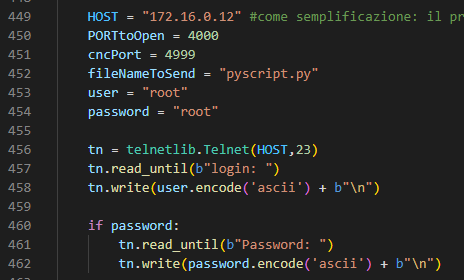
\includegraphics[scale=0.5]{UNINA_MSc_Thesis_Project/img/Codice/loginTelnet.png}
    \caption{Login Telnet - da documentazione ufficiale}
    \label{fig:my_label}
\end{figure}

In figura sono mostrati i comandi poi richiamati dal Loader/Scanner dopo aver effettuato l'accesso sulla macchina vittima.
\begin{figure}[H]
    \centering
    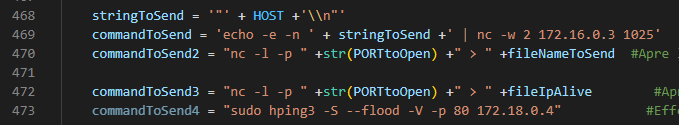
\includegraphics[scale=0.8]{UNINA_MSc_Thesis_Project/img/Codice/comandiTelnet.png}
    \caption{Comandi Telnet}
    \label{fig:my_label}
\end{figure}

Il ciclo, facente parte del main, si occupa di infettare tutti i nuovi bot, dopo la ricezione del comando di avvio da parte del Command and Control (CnC).
\begin{figure}[H]
    \centering
    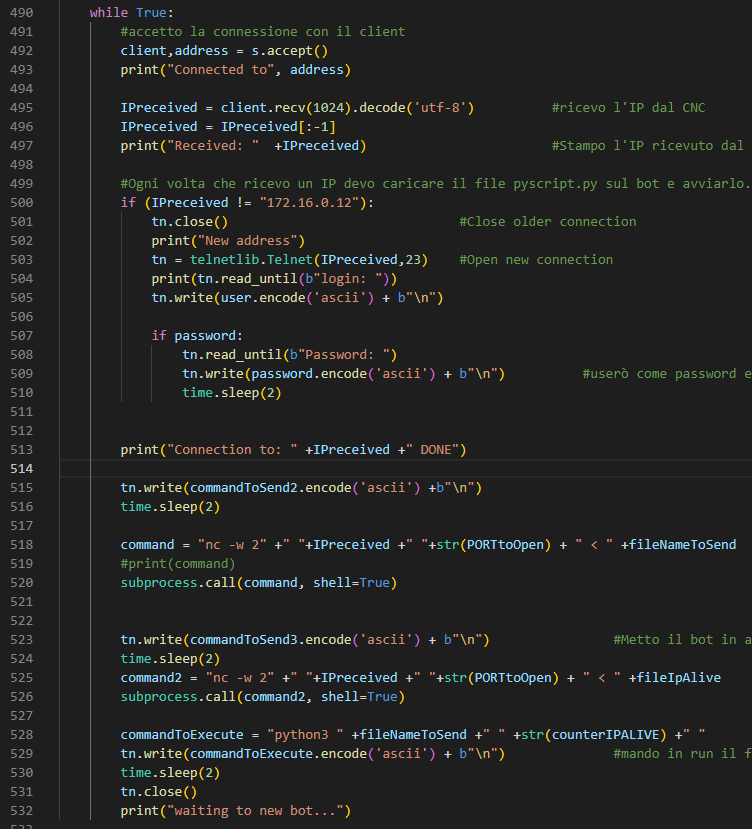
\includegraphics[scale=0.5]{UNINA_MSc_Thesis_Project/img/Codice/cicloLoading.png}
    \caption{nmapScan}
    \label{fig:my_label}
\end{figure}

Per poter funzionare, il CnC deve utilizzare due comandi: 

\begin{lstlisting}[language=Python]
nc -l -k -p 1025 >> vulnerableIP.txt
\end{lstlisting}

Che riceve in input l'indirizzo IP infettato, inviato dallo stesso nodo infetto e lo salva sul file $vulnerableIP.txt$

\begin{lstlisting}[language=Python]
tail -F vulnerableIP.txt | nc -w 2 172.16.0.4 4999
\end{lstlisting}

Che si occupa di inviare, ad ogni nuovo aggiornamento del file $vulnerableIP.txt$, il nuovo IP allo scanner alla porta 4999 in ascolto.

\section{Esecuzione dell'attacco}
L'attacco funziona in questo modo: 
\begin{enumerate}
    \item Lo scanner tenta il login con le credenziali root-root
    \item Il login è riuscito: viene inviato, da parte del bot, il proprio IP al CnC.
    \item Il CnC invia l'indirizzo IP del bot da attaccare 
    \item Lo scanner effettua il login, carica lo script python $pyscript.py$ e lo esegue, tramite telnet.
    \item Lo script, piuttosto che lo scanner, cerca nuovi bot, come da punto 1
    \item Trovato un bot vulnerabile, invia l'IP del nuovo bot, tramite il bot infetto, al CnC
    \item Il CnC invia l'IP della macchina vulnerabile allo scanner
\end{enumerate}

\subsection{Docker Security Playground}
In figura è presente lo schema grafico prodotto con Docker Security Playground ottenuto con il motore grafico DSP. 
\begin{figure}[H]
    \centering
    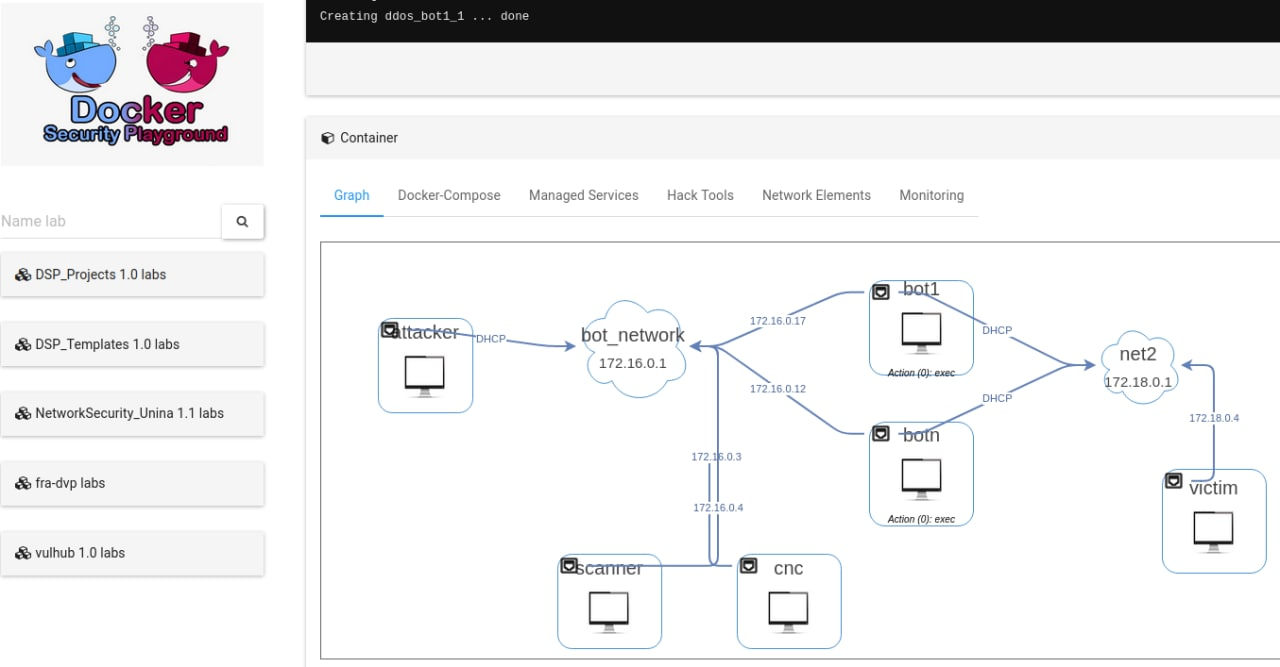
\includegraphics[scale=0.3]{UNINA_MSc_Thesis_Project/img/Esecuzione/DSP Schema.jpg}
    \caption{Schema Docker Security Playground}
    \label{fig:my_label}
\end{figure}
Sono presenti due reti:
\begin{enumerate}
    \item bot network: 172.16.0.1
    \item net2 (rete della vittima): 172.18.0.1
\end{enumerate}




\subsection{Diagramma di sequenza}
Il diagramma descrive lo scenario in cui, una volta tentato l'accesso con le credenziali root-root, vi è il login riuscito e si prosegue al caricamento dello script malevolo sul bot che, a sua volta, inonda di richiesta il server vittima.

\begin{figure}[H]
    \centering
    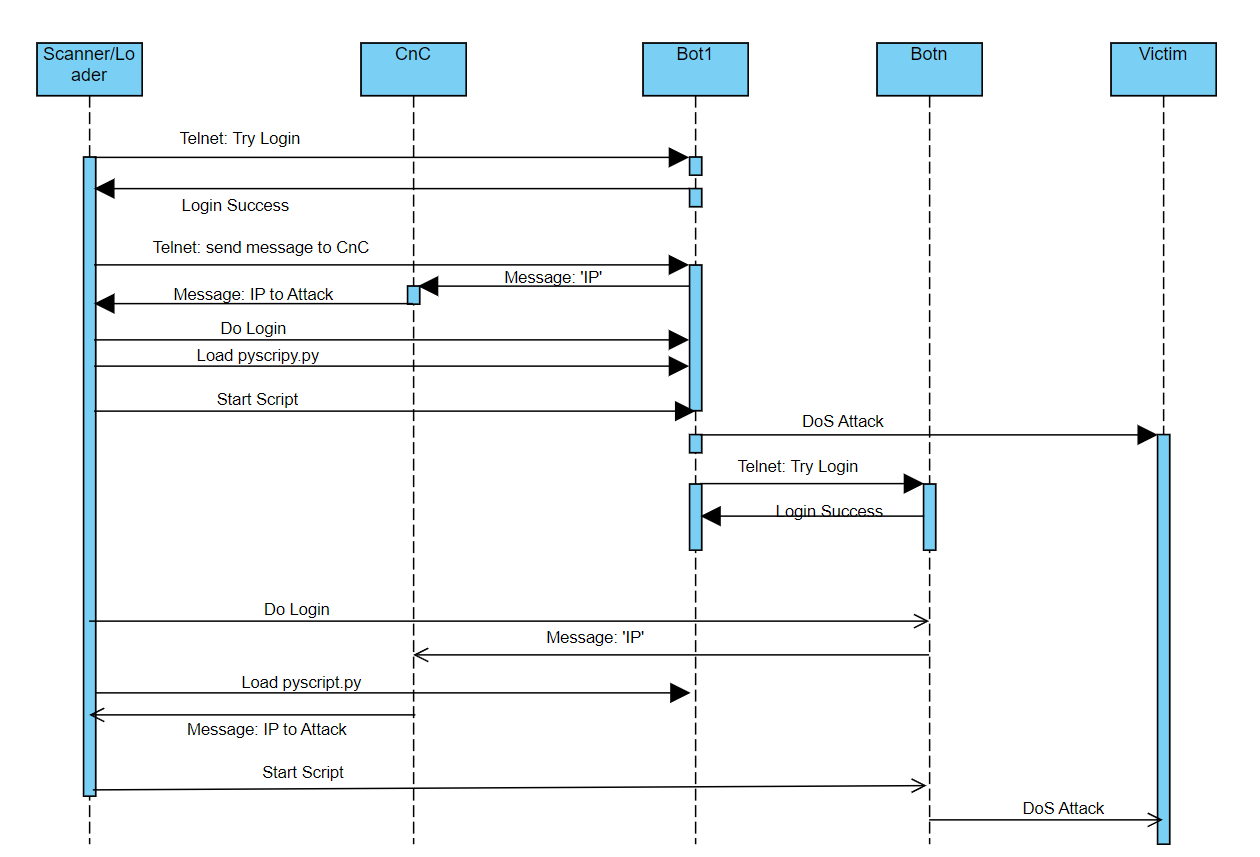
\includegraphics[scale=0.5]{UNINA_MSc_Thesis_Project/img/Esecuzione/sequence_attack.png}
    \caption{Diagramma di sequenza dell'attacco}
    \label{fig:my_label}
\end{figure}

\subsection{Risultati Ottenuti}
All'avvio dello script python, la linea di comando si presenta come in figura. In questa fase vi è l'invio dell'indirizzo IP della macchina per permettere di trovare gli IP vivi nella rete.

\begin{figure}[H]
    \centering
    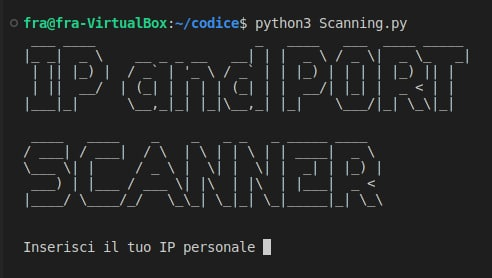
\includegraphics[scale=0.5]{UNINA_MSc_Thesis_Project/img/Esecuzione/Scanning_start.jpg}
    \caption{Start dello script}
    \label{fig:my_label}
\end{figure}

Il risultato ottenuto si presenta come in figura. Gli IP vivi nella rete sono:

\begin{lstlisting}[language=Python]
172.16.0.12
172.16.0.17
\end{lstlisting}

Ovvero i due IP dei bot all'interno della rete. Il Risultato di output si presenta come in figura: 

\begin{figure}[H]
    \centering
    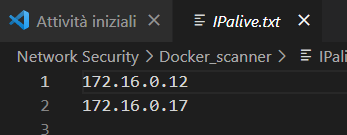
\includegraphics[scale=0.8]{UNINA_MSc_Thesis_Project/img/Esecuzione/ipalive.png}
    \caption{ipalive.txt}
    \label{fig:my_label}
\end{figure}

Superata la prima fase, vi è la fase di scelta dello Scanner da utilizzare, che si presenta come in figura. Per la scelta è necessario selezionare il numero e cliccare invio.

\begin{figure}[H]
    \centering
    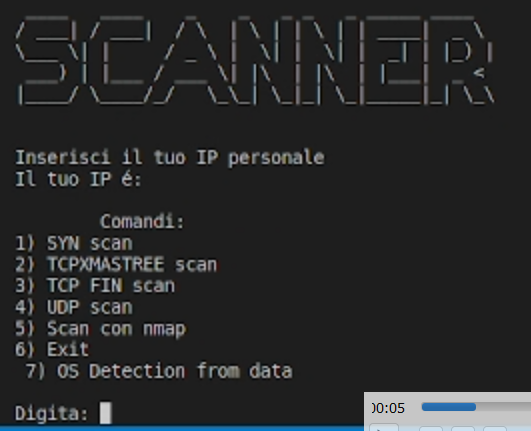
\includegraphics[scale=0.5]{UNINA_MSc_Thesis_Project/img/Esecuzione/ScanningChoice.png}
    \caption{Scelta del tipo di scan da effettuare}
    \label{fig:my_label}
\end{figure}

I risultati dello scanner sono come mostrati. Sono presenti gli indirizzi IP e le loro porte risultate apert separate con uno "-".

\begin{lstlisting}[language=Python]
172.16.0.12-23
172.16.0.17-23
\end{lstlisting}

Il risultato ottenuto:

\begin{figure}[H]
    \centering
    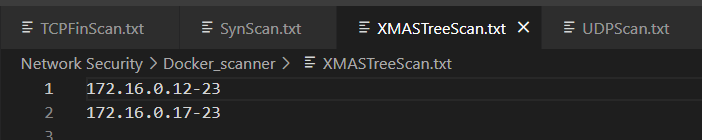
\includegraphics{UNINA_MSc_Thesis_Project/img/Esecuzione/scannerResults.png}
    \caption{Risultati dello scanning}
    \label{fig:my_label}
\end{figure}

In figura anche uno scan, ottenuto col bot, di un computer Windows (tramite scansione con Virtualbox):
\begin{figure}[H]
    \centering
    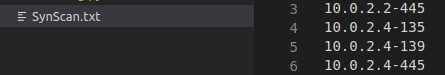
\includegraphics[scale=0.6]{UNINA_MSc_Thesis_Project/img/Esecuzione/SynScan Windows.jpg}
    \caption{SYN scan su windows}
    \label{fig:my_label}
\end{figure}

In figura sono presenti i due file "IPalive.txt" e "pyscript.py" ricevuti dai due bots.
\begin{figure}[H]
    \centering
    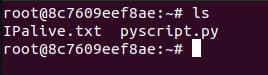
\includegraphics{UNINA_MSc_Thesis_Project/img/Esecuzione/bot1_received.jpg}
    \caption{I due files ricevuti dal bot 1 durante l'attacco}
    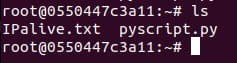
\includegraphics{UNINA_MSc_Thesis_Project/img/Esecuzione/bot2_received.jpg}
    \caption{I due files ricevuti dal bot 2 durante l'attacco}
    \label{fig:my_label}
\end{figure}

Il comando per effettuare un attacco DoS, da parte di ogni singolo bot è:

\begin{lstlisting}[language=Python]
hping3 -S --flood -V -p 80 172.18.0.4
\end{lstlisting}

hping3 è uno strumento di rete in grado di inviare pacchetti TCP/IP personalizzati per effettuare attacchi informatici.

Dalla man-page linux: 
\begin{lstlisting}[language=Python]
hping3 [ -hvnqVDzZ012WrfxykQbFSRPAUXYjJBuTG ] [ -c count ] [ -i wait ] [ --fast ] [ -I interface ] [ -9 signature ] [ -a host ] [ -t ttl ] [ -N ip id ] [ -H ip protocol ] [ -g fragoff ] [ -m mtu ] [ -o tos ] [ -C icmp type ] [ -K icmp code ] [ -s source port ] [ -p[+][+] dest port ] [ -w tcp window ] [ -O tcp offset ] [ -M tcp sequence number ] [ -L tcp ack ] [ -d data size ] [ -E filename ] [ -e signature ] [ --icmp-ipver version ] [ --icmp-iphlen length ] [ --icmp-iplen length ] [ --icmp-ipid id ] [ --icmp-ipproto protocol ] [ --icmp-cksum checksum ] [ --icmp-ts ] [ --icmp-addr ] [ --tcpexitcode ] [ --tcp-timestamp ] [ --tr-stop ] [ --tr-keep-ttl ] [ --tr-no-rtt ] [ --rand-dest ] [ --rand-source ] [ --beep ] hostname
\end{lstlisting}

Andando a vedere nel dettaglio ogni singola opzione:
\begin{itemize}
    \item -S: Syn flood
    \item flood: Invia pacchetti nel modo più veloce possibile senza mostrare le risposte in ingresso 
    \item -V: modalità verbose 
    \item -p: porta dell'attacco (porta 80)
\end{itemize} 

\subsection{codice dello script $pyscript.py$}
Il codice dello script pyscripy.py è tratto da $Scanning.py$ e si occupa di:
\begin{itemize}
    \item Login telnet
    \item Invio, da parte del bot infetto, dell'IP personale.
\end{itemize}

